\documentclass[10pt,journal,compsoc]{IEEEtran}
\usepackage[spanish]{babel}
\usepackage{listings}
\usepackage{graphicx}
\usepackage{wrapfig}
\usepackage{lipsum}
\ifCLASSOPTIONcompsoc
  \usepackage[nocompress]{cite}
\else
  \usepackage{cite}
\fi

\ifCLASSINFOpdf
\else
\fi
\newcommand\MYhyperrefoptions{bookmarks=true,bookmarksnumbered=true,
pdfpagemode={UseOutlines},plainpages=false,pdfpagelabels=true,
colorlinks=true,linkcolor={black},citecolor={black},urlcolor={black},
pdftitle={Pascal},
pdfsubject={Lenguaje de Progemaci\'on Pascal},
pdfauthor={Daniel, Wilbert, Anthony, Bryan},
}
\renewcommand{\lstlistingname}{Cuadro}
\lstset{
	extendedchars=true,
	frame = single, 
	language=Pascal, 
	framexleftmargin=3pt
}
\hyphenation{op-tical net-works semi-conduc-tor}


\begin{document}
\title{Pascal}

\author{Daniel~Delgado,~\IEEEmembership{Estudiante,~ITCR,}
	Wilbert~Gonzales,~\IEEEmembership{Estudiante,~ITCR,}
	Anthony~Leandro,~\IEEEmembership{Estudiante,~ITCR,}
	and~Bryan~Mena,~\IEEEmembership{Estudiante,~ITCR}
}
\markboth{Lenguajes de Programaci\'on, Tarea Corta 2, Agosto 2017}
{Shell \MakeLowercase{\textit{et al.}}: \LaTex}


\maketitle

\IEEEdisplaynontitleabstractindextext

\IEEEpeerreviewmaketitle

\section{Datos Historicos}
\begin{wrapfigure}{R}{0.3\textwidth}
	\centering
	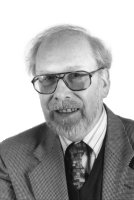
\includegraphics[width=0.25\textwidth]{wirth.jpg}
	\caption{\label{fig:NiklausWirth}Niklaus Wirth.}
\end{wrapfigure}
Pascal fue creado en 1970 por Niklaus Wirth. Inicialmente estaba destinado a ser usado para ense\~nar a programar aunque su uso no se limita a esto, se han creado varias aplicaciones y videojuegos para PC como por ejemplo Dev-C++ y Skype los cuales fueron desarrollados, en parte, con Delphi (Object Pascal, una versi\'on un poco m\'as moderna de Pascal que implementa la Orentaci\'on a Objetos) adem\'as de sistemas embebido (sistema dise\~nado para realizar pocas funciones especificas en un sistema de manera constante) y fue ampliamente utilizado para desarrollo del computador Apple Lisa, Pascal estaba dise\~nado de manera que compilar mentalmente un programa se hiciera f\'acil esto debido a que el acceso a computadoras en aquella \'epoca era muy costoso. Cabe mencionar que la implementaci\'on de Orientaci\'on a Objetos de Pascal fue inicialmente desarrollada por Apple en 1986 pero fue hasta 1993 que Pascal Standards Committee  publica la extenci\'on de OO para Pascal

\section{Tipos de Datos}
En Pascal se utiliza la palabra \emph{type} cuando se va a realizar una declaraci\'on de un tipo para asignarle la semantica al tipo (tipo de dato, rango de dato, operaciones posibles). Adem\'as, es importante recalcar que no todas las distribuciones de pascal soportan los mismos tipos de datos, por ejemplo, pascal estandar no posee soporte para cadenas de caracteres, aunque FreePascal lo hace 
\begin{tabular}{ l r r r }
	Nombre & Tipo de Dato & Ejemplo \\
	\hline\\
	String & Texto & 'Lenguajes'\\
	Integer & N\'umeros Enteros & 6, 3545 \\
	Real & N\'umeros Decimales & 3.14, 15.6\\
	Boolean & Valor Booleano & TRUE, FALSE \\
	Character & Un \'unico car\'acter & 'V', 'B'\\
	Enumerados &  -- & ver cuadro1\\
	Record & Datos heterogeneos & ver cuadro1\\
\end{tabular}\\\newline\newline\newline
\begin{lstlisting}[language=Pascal, caption = {C\'odigo de tipo de datos enumerados y de registro en Pascal}][linewidth=5.4cm]
type
//TipoMes Enumerado
TipoMes = (Ene, Feb, Mar, Abr, May, 
Jun, Jul, Ago, Sep, Oct, Nov, Dec)
//TipoFecha y Cita Record
TipoFecha = record
Mes : TipoMes;
Dia : 1..3; //Subrangos, Revisar seccion 2.3
A\~no : 1900..2000;
end;
Cita = record
Fecha : TipoFecha;
Hora : 0..2400;
end;
\end{lstlisting}

\subsection{Enumerated}
Define un rango de elementos a los que se refieren los identificadores(Ver cuadro 2). Es posible definir subrangos de ellos. Puesto que son ordenados, pueden compararse entre s\'i. Funciones aplicables a un identificador de un tipo Enumerated:\footnote{Datos tomados de www.gnu-pascal.de. Ver Refencias [7]}
\begin{enumerate}
	\item Ord: Cantidad de ocurrencias de un identificador
	\item Pred y Succ: Predecesor y sucesor de un identificador
\end{enumerate}
\begin{lstlisting}[language=Pascal, caption = {C\'odigo de declaraci\'on en enumerated}][linewidth=5.4cm]
type
<Nombre Tipo> = 
    (<identificador>,...,<identificador>);
\end{lstlisting}

\subsection{Arrays}
\begin{lstlisting}[language=Pascal, caption = {C\'odigo de declaraci\'on para un array}][linewidth=5.4cm]
type
typename = 
	array [<Rango>] of <Tipo Dato>;
\end{lstlisting}

\subsection{Punteros}
Como en C o C++ un puntero es una direcci\'on a memoria, de manera similar es necesario indicar a que tipo de dato se apuntar\'a, en pascal esto se hace poniendo el car\'acter \large \textasciicircum~ \normalsize antes del tipo de variable a la que se desea apuntar, luego se debe asignar un espacio en memoria que ser\'a donde el puntero viva, esto se hace con el comando New(Nombre\_Puntero),~aclarando que el puntero es de tipo puntero a un tipo de dato, para asignarle un valor al espacio de memoria al cual se esta apundando se necesita utilizar de nuevo el car\'acter \large \textasciicircum~ \normalsize y asignar el valor, como ejemplo proponemos una lista implementada por medio de punteros:
\begin{lstlisting}[language=Pascal, caption = {C\'odigo de una lista con punteros}][linewidth=5.4cm]
type
	punteroNodo = ^Nodo;	
	Nodo = record
	dato : integer;
	siguiente : punteroNodo;
end;
\end{lstlisting}

\subsection{Subrangos}
Puede asociarsele con un "slice", toma un objeto y recupera la informaci\'on desde Menor\_Valor..Mayor\_Valor, a continuaci\'on se presenta un ejemplo se subrangos con un tipo Enumerated:
\begin{lstlisting}[language=Pascal, caption = {Ejemplo de subrangos}][linewidth=3.5cm]
type
Meses = (Enero, Febrero, Marzo, Abril
Mayo, Junio, Julio, Agosto,
Septiembre, Octubre, Noviembre,
Diciembre);
Subrango = Enero..Abril;
\end{lstlisting}

\subsection{Puntos Importantes\protect\footnote{Datos Obtenidos de \emph{Pascal Data Types and Variables}, Computer Science Department at New York University}}
\begin{itemize}
	\item Cuando se declara un string se le asigna una longitud m\'axima, de no asignarsele una el valor por defecto es de 255
	\item Para el nombre de las variables se siguen estos principios:
	\subitem *Debe empezar con una letra o un underscore(\verb|_|)
	\subitem *No puede tener espacios en blanco
	\subitem *Los car\'acteres permitidos son letras, n\'umeros o underscore
\end{itemize}
A continuaci\'on se presentan algunos de los rangos para Integers, igualmente cabe la aclaraci\'on que no todos los compiladores ni distribuciones de pascal son iguales, por lo tanto pueden existir inconsistencias en los siguientes datos:
\begin{tabular}{c p{5cm} p{1cm}}
	Tipo & Rango & Bits\\
	\hline\\
	Byte & 0..255 & 8\\
	\hline\\
	Shortint & -128..127 & 8\\
	\hline\\
	Integer & -32768..32767 & 16\\
	\hline\\
	Word & 0..65535 & 16\\
	\hline\\
	Cardinal & 0..2147483647 & 32\\
	\hline\\
	Longint & -2147483648..2147483647 & 32\\
	\hline\\
	Single & $1.5x10^{-45}$..$3.4x10^{38}$ & 32\\
	\hline\\
	Real & $2.9x10^{-39}$..$1.7x10^{38}$ & 48\\
	\hline\\
	Double & $5x10^{-324}$..$1.7x10^{308}$ & 64\\
	\hline\\
	Extended & $3.4x10^{-4932}$..$1.1x10^{4932}$ & 80\\
	\hline\\
	Comp & -9223372036854775809.. & 64\\
	     & 9223372036854775807 &     \\
	\hline\\
\end{tabular}

\section{Estructuras de control y Expresiones}
En Pascal se utilizan bloques de codigo, inician con un \emph{begin} y terminan con un \emph{end}. Como dato curioso en Pascal \emph{end} no necesariamente termina en ";", al contrario cuando se utiliza para terminar un archivo de pascal se utiliza un "."\\
Ejemplo:
\begin{lstlisting}[language=Pascal, caption = {C\'odigo Hola Mundo en Pascal}][linewidth=5.0cm]
program Hola;
begin
	writeln("Hola Mundo");
end.
\end{lstlisting}

\subsection{Estructura t\'ipica de un programa}
\begin{lstlisting}[language=Pascal, caption = {Estructura t\'ipica de un programa en Pascal}][linewidth=5.0cm]
PROGRAM <Nombre del programa> (FileList);

CONST
	<Declarar Constantes>
	
TYPE
	<Declarar Tipos>
	
VAR
	<Declarar Variables>
	
BEGIN
	<Expresiones Ejecutables>
END.
\end{lstlisting}

\subsection{Constantes}
Definidas en el bloque de constantes al inicio del programa, se utilizan identificadores para referenciarlas, el valor que almacenan no podr\'a ser cambiado a lo largo del programa
\begin{lstlisting}[language=Pascal, caption = {Declaraci\'on de Constantes}][linewidth=5.0cm]
const
	Identificador1 = value;
	Identificador2 = value;
	Identificador3 = value;
	//...
\end{lstlisting}

\subsection{Variables}
\begin{lstlisting}[language=Pascal, caption = {Declaraci\'on de Variables}][linewidth=5.0cm]
var
	Identificador1 : DataType1;
	Identificador2 : DataType2;
	Identificador3 : DataType3;
	//...
\end{lstlisting}
Cabe mencionar que los identificadores pueden ser "listas", o sea, varios identificadores separados por comas que ser\'an declarados del mismo tipo

\subsection{Tipos}
\begin{lstlisting}[language=Pascal, caption = {Declaraci\'on de Tipos}][linewidth=5.0cm]
type
	Identificador1 = <Type Definition>;
	Identificador2 = <Type Definition>;
	//...
\end{lstlisting}

\subsection{Identaci\'on y Puntuaci\'on}
Es necesario utilizar puntuaci\'on para decirle al compilador cuando un \emph{statement} termina. Se utiliza \emph{;} en las siguientes situaciones:
\begin{itemize}
	\item Despues de la declaraci\'on del programa
	\item Despues de cada definici\'on de constante
	\item Despues de cada definici\'on de variable
	\item Despues de cada definici\'on de tipo
	\item Despues de cada \emph{statement}
\end{itemize}

\subsection{Comentarios en el c\'odogo}
A lo largo del tiempo en Pascal se han implementado diferentes maneras de comentar en el c\'odogo, el comentario cl\'asico inicia con (* y termina con *), lo anterior para comentarios de una sola l\'inea,para comentarios multil\'inea se utilizan los \{\}, otras versiones de Pascal, por ejemplo Delphi, utilizan // para comentarios de una l\'inea 

\subsection{Recursi\'on}
Como es necesario para un lenguaje de programaci\'on en Pascal es posible utilizar la recursi\'on, importante recordar utilizar una condici\'on de parada en la recursi\'on para evitar que esta se vuelva infinita, seguidamente se presenta un ejemplo del uso de la recursi\'on para resolver una suma:
\begin{lstlisting}[language=Pascal, caption = {Recursi\'on en Pascal}][linewidth=5.0cm]
function Suma (num : integer) : integer;
begin
	if num = 1 then 
		Suma := 1
	else 
		Suma := Suma(num-1) + num
end;
\end{lstlisting}

\subsection{Estatutos \emph{IF}}
\begin{lstlisting}[language=Pascal, caption = {Sintaxis de un IF}][linewidth=5.0cm]
var X, Y: Integer;
BEGIN
Writeln ("Digite dos numeros: ");
Readln (X,Y);
if (X >Y) then
	Writeln (X, " Es mayor que ",Y)
else
	Writeln (X, " Es menor que ", Y);
end.
\end{lstlisting}

\subsection{Estatutos \emph{CASE}}
\begin{lstlisting}[language=Pascal, caption = {Sintaxis de un Case}][linewidth=5.0cm]
Case <Caso> OF
<Caso con valor 1>: <Hacer ... 1>;
<Caso con valor 2>: <Hacer ... 2>;
...
Else
	<Hacer ... n>
End;
\end{lstlisting}

\subsection{Estatutos \emph{WHILE}}
\begin{lstlisting}[language=Pascal, caption = {Sintaxis de un While}][linewidth=5.0cm]
While (Conditional Expression) do
	<Hacer...>;
\end{lstlisting}

\subsection{Estatutos \emph{REPEAT}}
\par Parecido al estatuto while, la diferencia recae en que primero realiza los estatutos declarados en su bloque y luego pregunta la condici\'on booleana (Hacer luego preguntar)
\begin{lstlisting}[language=Pascal, caption = {Sintaxis de un Repeat}][linewidth=5.0cm]
Repeat
	<Hacer...>;
Until (Conditional Expression)
\end{lstlisting}

\subsection{Estatutos \emph{FOR}}
El estatuto for es utilizado cuando se conoce el numero exacto de repeticiones de un ciclo. Existen dos maneras de utilizarlo, desde el inicio hasta el final o desde el final hasta el inicio
\begin{lstlisting}[language=Pascal, caption = {Sintaxis de un FOR}][linewidth=5.0cm]
//Inicia el for desde el 
//valor inicial hasta el valor final
FOR <Variable> := <Inicio> TO <Final> DO
	<Hacer...>;

//Inicia el for desde el 
//valor final hasta el valor incial
FOR <Variable> := <Final> DOWNTO <Inicio> DO
	<Hacer...>;
\end{lstlisting}
\vspace{0.5cm}
En 2005 Delphi implementa una nueva forma de realizar un \emph{for} (similar al \emph{for} en Python). Ejemplo
\begin{lstlisting}[language=Pascal, caption = {Sintaxis de un FOR en Delphi}][linewidth=5.0cm]
begin
for <varName> in <ObjIterable> do
	<Hacer...>
end;
\end{lstlisting}

\vspace{0.7cm}

\subsection{Estatutos \emph{WITH}}
Utilizado para accesar a las propiedades de un Record sin tener que referenciar al Record constantemente. Ejemplo:
\begin{lstlisting}[language=Pascal, caption = {Sintaxis de un WITH}][linewidth=3.0cm]
with date do
	if month = 12 then
		begin 
			month := 1 ; 
			year := year + 1
		end
	else 
		month := month+1
\end{lstlisting}
El c\'odigo anterior remplaza el siguiente, eliminando la necesidad de referirse al Record cada vez que se va a accesar a alguno de sus campos.\footnote{Ejemplos tomados del documento ISO 7185:1990 ver [6]}
\begin{lstlisting}[language=Pascal]
if date .month = 12 then
	begin 
		date .month := 1 ; 
		date .year := date .year+1
	end
else 
	date .month := date .month+1
\end{lstlisting}

\subsection{Procedures}
\begin{lstlisting}[language=Pascal, caption = {Sintaxis de un Procedure}][linewidth=3.0cm]
procedure <Nombre>(Lista de parametros);
	<Declaracion de constantes locales>
	<Declaracion de variables locales>
	begin
		<Hacer...>
	end;
\end{lstlisting}
Para llamar un procedure se utiliza su nombre m\'as los datos para satisfacer la lista de parametros declarados. 

\subsection{Funciones}
Cabe aclarar que funciones y Procedures no son lo mismo, procedures son un conjunto de instrucciones que se ejecutan cuando se llaman, las funciones son lo mismo, la diferencia recae en que las funciones tienen valores de retorno mentras que los procedures no.
\begin{lstlisting}[language=Pascal, caption = {Sintaxis de una funci\'on}][linewidth=3.5cm]
function <Nombre>(Parametros):<TipoRetorno>;
	<Declaracion de constantes locales>
	<Declaracion de variables locales>
	begin
		<Hacer...>;
		<Nombre>: = return <Valor>;
	end;
\end{lstlisting}

\subsection{Operadores Booleanos}
\begin{tabular}{c p{6cm} p{15cm}}
	Operador & Significado\\
	\hline\hline
	$and$ & Las dos condiciones evaluadas tienen que ser verdad\\\hline
	$and~then$ & Igual que $and$ solo que garantiza que se evalueen las expresiones en el orden dado\\\hline
	$or$ & Al menos una de las condiciones debe ser verdad\\\hline
	$or~else$ & Igual que $or$ solo que garantiza que se evalueen las expresiones en el orden dado\\\hline
	$not$ & Niega el resultado\\\hline
	$xor$ & $or$ exclusivo\\ 
	\hline 
\end{tabular}

\subsection{Operadores condicionales}
Es importante mencionar que la asignaci\'on en Pascal es "$:=$", y, como se muestra en el siguiente cuadro la condicional de igualdad es "$=$"\newline\newline
\begin{tabular}{c p{3cm} p{5cm}}
	Operador & Significado\\
	\hline\hline\\
	$=$ & Igualdad\\
	$>$ & Mayor que\\
	$<$ & Menor que\\
	$>=$ & Mayor Igual que\\
	$<=$ &Menor Igual que\\
	$<>$ & Diferente\\
	\hline
\end{tabular}

\subsection{Operadores Aritmeticos}
\begin{tabular}{p{1.2cm} p{1.78cm} p{1.4cm} p {2.5cm}}
	Operador & Operaci\'on & Operandos & Tipo Resultado\\
	\hline\\
	+ & Suma & Integer o Real & Integer si los dos operandos son integer, real de otra forma\\\hline\\
	- & Resta & Integer o Real & Integer si los dos operandos son integer, real de otra forma\\\hline\\
	$*$ & Multiplicaci\'on & Integer o Real & Integer si los dos operandos son integer, real de otra forma\\\hline\\
	/ & Divisi\'on & Integer o Real & Real\\\hline\\
	div & Divisi\'on truncada & Integer & Integer\\\hline\\
	mod & Modulo & Integer & Integer\\\hline\\
\end{tabular}

\subsection{Prioridad de algunas operaciones}
\begin{enumerate}
	\item $not$
	\item  $*,~/,~div,~mod,~and$
	\item $+,~-,~or$
	\item $<~>~<=~>=~=~<>$
\end{enumerate}

\section{Caracter\'isticas}
\begin{itemize}
	\item Case Insensitive
	\item Lenguaje fuertemente tipado(Una variable es y ser\'a del tipo que se le declara y esto no se puede cambiar)
	\item Algunos compiladores solo le dan importancia a los primeros 32 car\'acteres (aproximadamente) de un identificador
\end{itemize}

\section{Caracter\'isticas y Ventajas}
\begin{itemize}
	\item Legible, es un lenguaje con una sintaxis que se asemeja mucho al ingl\'es, esto hace que el c\'odigo en Pascal sea mucho m\'as f\'acil de aprender y de leer
	\item Variedad de estructuras de control y tipos de datos
	\item Versiones m\'as modernas soportan la orientaci\'on a objetos
\end{itemize}


\section{Desventajas}
\begin{itemize}
	\item Popularidad: Pascal no es un lenguaje tan popular como lo puede ser Java u otros, esto conduce a que librerias y otros aditivos sean escasos para solucionar cierto tipo de problemas
	\item Multiples Versiones sin un standard bien definido: esto hace que migrar aplicaciones de un ambiente a otro sea muy dificil incluso imposible, aun con versiones m\'as modernas como Delphi no hay un standard definido
\end{itemize}

\begin{thebibliography}{3}
	
	\bibitem{Pascal}
	N.~Wirth \emph{Recollections about the development of Pascal.} In The second ACM SIGPLAN conference on History of programming languages (HOPL-II). ACM, New York, NY, USA, 333-342. DOI=http://ezproxy.itcr.ac.cr:2075/10.1145/154766.155378
	
	\bibitem{Pascal2}
	N.~Wirth. 1975. \emph{An assessment of the programming language PASCAL.} In Proceedings of the international conference on Reliable software. ACM, New York, NY, USA, 23-30. DOI=http://ezproxy.itcr.ac.cr:2075/10.1145/800027.808421
	
	\bibitem{Pascal3}
	N. Wirth. 1976. Comment on a note on dynamic arrays in PASCAL. SIGPLAN Not. 11, 1 (January 1976), 37-38. DOI=http://ezproxy.itcr.ac.cr:2075/10.1145/987324.987330
	
	\bibitem{Pascal4}
	N.~Wirth \emph{The Programming Language Pascal} Acta Informatica, Vol. 1, Fasc. 1, 1971 pp. 35-63
	
	\bibitem{PascalDesventajas}
	B.~Kernighan 1981 \emph{Why Pascal is Not My Favorite Programming Language} Recuperado de:
	http://www.lysator.liu.se/c/bwk-on-pascal.html
	
	\bibitem{Pascal5}
	Pascal ISO 7185:1990 Recuperado de: https://www.iso.org/obp/ui/\#iso:std:iso:7185:ed-2:v1:en
	
	\bibitem{Pascal6}
	\emph{The GNU Pascal Manual} Recuperado de: http://www.gnu-pascal.de/gpc/
	
\end{thebibliography}

\end{document}


